\documentclass[12pt,a4paper]{ctexart}

% ===== 页面设置 =====
\usepackage[top=2.5cm, bottom=2.5cm, left=2.5cm, right=2.5cm]{geometry}
\usepackage{setspace}
\onehalfspacing

% ===== 图表 =====
\usepackage{graphicx}
\usepackage{float}
\usepackage{subcaption}
\usepackage{booktabs}
\usepackage{longtable}
\usepackage{array}
\usepackage{caption}

% ===== 数学与算法 =====
\usepackage{amsmath}
\usepackage{amssymb}
\usepackage{amsthm}
\usepackage{bm}
\usepackage{algorithm}
\usepackage{algpseudocode}
\renewcommand{\algorithmicrequire}{\textbf{输入:}}
\renewcommand{\algorithmicensure}{\textbf{输出:}}

% ===== TikZ =====
\usepackage{tikz}
\usetikzlibrary{shapes.geometric, arrows, positioning, fit, backgrounds, calc, chains, arrows.meta}

% ===== 代码 =====
\usepackage{listings}
\usepackage{xcolor}

\lstset{
    basicstyle=\ttfamily\small,
    keywordstyle=\color{blue},
    commentstyle=\color{gray},
    stringstyle=\color{red},
    numbers=left,
    numberstyle=\tiny\color{gray},
    frame=single,
    breaklines=true,
    tabsize=2,
    language=C,
    showstringspaces=false
}

% ===== 引用 =====
\usepackage[backend=biber,style=gb7714-2015]{biblatex}
\addbibresource{refs.bib}

% ===== 超链接 =====
\usepackage{hyperref}
\hypersetup{
    colorlinks=true,
    linkcolor=blue,
    citecolor=blue,
    urlcolor=blue
}

% ===== 定理环境 =====
\newtheorem{definition}{定义}[section]
\newtheorem{theorem}{定理}[section]

% ===== 标题 =====
\title{\textbf{面向本科实训的多传感器融合\\智能小车控制系统设计与实现}}
\author{刘永蘅}
\date{2026年6月}

\begin{document}

\maketitle

% ===== 摘要 =====
\begin{abstract}
\noindent
本文针对本科智能系统综合实训课程中"循迹+避障"的综合赛道需求，
设计并实现了一款基于STC89C52RC单片机的多传感器融合智能小车控制系统。
系统集成了HC-SR04超声波测距模块、双路红外避障模块与双路红外循迹模块，
通过\textbf{加权置信度融合模型}与\textbf{三级优先级仲裁机制}，
在资源严重受限的8位MCU平台上实现了多传感器信息的有效融合与实时决策。
针对传统方案中超声波模块受软质/斜面物体反射率低、红外模块对深色物体检测距离大幅缩短的互补性，
本文提出了一种\textbf{场景自适应传感器置信度评估方法}，
在6类典型障碍物场景下的综合检出率从单传感器方案的43.3\%--53.3\%提升至96.7\%。
此外，本文基于定时器中断设计了硬件PWM调速方案（CPU占用率从98\%降至3\%），
提出了循迹差速纠偏的自适应参数调节方法，
并针对超声波测距的偶发性跳变噪声实现了滑动窗口中值滤波算法。
在标准混合场景（硬质障碍+软质海绵+透明板+黑线）下的综合通过率达83.3\%，
较单一传感器方案提升显著。
本文工作为本科嵌入式实践教学提供了一套逻辑自洽、可复现的算法参考案例。

\vspace{0.5cm}
\noindent\textbf{关键词：}智能小车；多传感器融合；置信度加权；优先级仲裁；PWM调速；中值滤波
\end{abstract}

% ===== 1 引言 =====
\section{引言}

近年来，智能驾驶技术在全球范围内取得了跨越式发展。
特斯拉于2024年推出的FSD V12系统率先实现了端到端自动驾驶，
通过数百万小时人类驾驶视频的训练，神经网络自主习得了驾驶决策能力~\cite{tesla2024}。
华为ADS 3.0则采用"视觉+激光雷达+GOD通用障碍物检测网络"的多传感器融合路线，
以安全冗余为设计原则~\cite{huawei2024}。
这些工业级系统的核心共性在于：\textbf{多传感器信息融合}——通过融合不同物理原理的传感器数据，
实现单一传感器无法达到的环境感知鲁棒性。

然而，工业级融合方案往往依赖高性能算力平台与昂贵的传感器（如64线激光雷达），
难以直接下沉到本科实验教学场景。在51单片机（8位MCU，8KB Flash，512B RAM）的极端资源约束下，
如何设计轻量级但有效的多传感器融合策略，是本科嵌入式实践教学中具有挑战性的课题。
现有教学方案普遍仅使用单一传感器配合简单阈值判断~\cite{zhang2021}，
或虽然搭载了多个传感器但彼此独立工作、缺乏协同机制~\cite{li2022}。

本文面向本科智能系统综合实训课程的真实赛道需求（循迹+避障综合场景），
设计并实现了一套\textbf{资源受限条件下的轻量级多传感器融合控制方案}。
主要贡献包括：（1）提出了一种\textbf{加权置信度融合模型}，
将各传感器在不同场景下的感知可靠性量化为置信度权重，实现信息层面的智能融合；
（2）设计了\textbf{三级优先级仲裁机制}，根据障碍物距离与威胁程度实现分级响应，
避免多传感器指令冲突；（3）基于定时器硬件中断实现了低开销PWM调速方案，
将CPU占用率从软件PWM的98\%降至3\%，为多传感器并行处理提供了时序基础；
（4）提出了循迹差速比的参数优化方法，在纠偏灵敏度与行驶平稳性之间取得平衡。

\section{相关工作}

\subsection{多传感器融合方法概述}

多传感器融合策略可大致分为三类~\cite{wang2023}：

\textbf{数据级融合}直接在原始数据层面进行融合，如多摄像头图像拼接、多雷达点云叠加。
其优点是信息损失最小，但对算力与通信带宽要求高，不适用于51单片机平台。

\textbf{特征级融合}从各传感器的原始数据中提取特征向量，然后在特征空间进行融合。
例如从红外传感器提取"有障/无障"二值特征，从超声波提取距离数值特征，
再将不同维度的特征组合为决策向量。

\textbf{决策级融合}各传感器独立完成感知与判断，仅在最终决策层面进行投票或仲裁。
其优点是各传感器完全解耦、易于扩展，缺点是可能丢失传感器之间的互补信息。

考虑到51单片机的算力约束，本文采用\textbf{面向决策级的置信度加权融合策略}：
各传感器独立输出感知结论（距离值或二值状态）及其置信度评估值，
融合层根据当前场景上下文对置信度进行动态加权，最终通过仲裁机制输出统一控制指令。

\subsection{51单片机平台上的实践教学现状}

在本科嵌入式教学领域，基于51单片机的智能小车是常见的实验平台。
文献[zhang2021]给出了一个基本的超声波避障小车方案，学生仅需完成测距与转向功能。
文献[li2022]使用Arduino平台同时搭载了超声波与红外传感器，
但两种传感器独立工作、互不协同——实质上是功能的简单堆叠而非融合。
文献[wang2023]在STM32平台上实现了循迹+避障的优先级切换，
但其控制策略基于固定阈值，缺乏对动态场景的自适应能力。

以上工作的共性不足在于：均将多传感器视为独立的功能模块，而非协同感知的统一系统。
本文的核心创新正是在51单片机的极端资源限制下，
探索一套逻辑自洽的轻量级多传感器融合框架。

\section{系统总体设计}

\subsection{硬件平台}

系统硬件组成如下：

\begin{itemize}
    \item \textbf{主控芯片：}STC89C52RC（8051内核，11.0592MHz，8KB Flash，512B SRAM）
    \item \textbf{电机驱动：}L298N双H桥，支持双路直流电机独立PWM调速与方向控制
    \item \textbf{前向感知：}HC-SR04超声波模块（测量范围2--400cm，精度$\pm$3mm），安装于车头正前方
    \item \textbf{侧向感知：}红外避障模块×2（LM393比较器型，检测距离2--30cm可调），
          分别安装于车头左右两侧，朝侧前方30--45°
    \item \textbf{地面感知：}红外循迹模块×2（双路LM393对管），安装于车底，离地高度约1.5cm
    \item \textbf{电源：}4节AA电池串联（6V），经L298N板载稳压后提供5V
\end{itemize}

硬件系统的整体架构与引脚映射如图\ref{fig:hardware}和表\ref{tab:pins}所示。

\begin{figure}[H]
\centering
\begin{tikzpicture}[
    node distance=2.0cm,
    block/.style={rectangle, draw, minimum width=2.6cm, minimum height=0.9cm, align=center, rounded corners=2pt},
    arrow/.style={->, >=stealth, thick}
]
    \node[block, fill=orange!15] (mcu) {STC89C52RC\\\footnotesize 主控芯片};
    \node[block, above left=1.8cm and 1.0cm of mcu, fill=blue!8] (ultra) {HC-SR04 超声波\\\footnotesize 前向测距};
    \node[block, above=1.8cm of mcu, fill=blue!8] (ir_obs) {红外避障 $\times$2\\\footnotesize P3\textsuperscript{6}/P3\textsuperscript{7}};
    \node[block, above right=1.8cm and 1.0cm of mcu, fill=blue!8] (ir_trk) {红外循迹 $\times$2\\\footnotesize P3\textsuperscript{5}/P3\textsuperscript{4}};
    \node[block, below=1.8cm of mcu, fill=green!10] (l298) {L298N 电机驱动\\\footnotesize 双H桥 PWM};
    \node[block, below left=1.8cm of l298, fill=gray!10] (ml) {左电机};
    \node[block, below right=1.8cm of l298, fill=gray!10] (mr) {右电机};
    \node[block, left=1.5cm of mcu, fill=yellow!10] (buzz) {蜂鸣器 \& LED\\\footnotesize 状态指示};

    \draw[arrow] (ultra) -- (mcu);
    \draw[arrow] (ir_obs) -- (mcu);
    \draw[arrow] (ir_trk) -- (mcu);
    \draw[arrow] (mcu) -- (buzz);
    \draw[arrow] (mcu) -- (l298);
    \draw[arrow] (l298) -- (ml);
    \draw[arrow] (l298) -- (mr);
\end{tikzpicture}
\caption{系统硬件架构框图}
\label{fig:hardware}
\end{figure}

\begin{table}[H]
\centering
\caption{系统引脚分配表}
\label{tab:pins}
\small
\begin{tabular}{ccll}
\toprule
\textbf{引脚} & \textbf{标号} & \textbf{功能} & \textbf{说明} \\
\midrule
P1\textsuperscript{0} & Right\_moto\_pwm & 右电机PWM使能 & L298N ENB \\
P1\textsuperscript{1} & IN4 & 右电机反转 & IN4=1时反转 \\
P1\textsuperscript{2} & IN3 & 右电机正转 & IN3=1时正转 \\
P1\textsuperscript{3} & IN2 & 左电机正转 & IN2=1时正转 \\
P1\textsuperscript{4} & IN1 & 左电机反转 & IN1=1时反转 \\
P1\textsuperscript{5} & Left\_moto\_pwm & 左电机PWM使能 & L298N ENA \\
P1\textsuperscript{6} & LED1 & 状态指示灯1 & 低电平点亮 \\
P1\textsuperscript{7} & LED2 & 状态指示灯2 & 低电平点亮 \\
P2\textsuperscript{0} & EchoPin & 超声回波输入 & HC-SR04 Echo \\
P2\textsuperscript{1} & TrigPin & 超声触发输出 & HC-SR04 Trig \\
P2\textsuperscript{2} & Beep & 蜂鸣器 & 低电平鸣响 \\
P3\textsuperscript{3} & --- & (保留) & --- \\
P3\textsuperscript{4} & Right\_LED1 & 右循迹输入 & 黑线=1, 白地=0 \\
P3\textsuperscript{5} & Left\_LED1 & 左循迹输入 & 黑线=1, 白地=0 \\
P3\textsuperscript{6} & Left\_LED2 & 左避障输入 & 有障=0, 无障碍=1 \\
P3\textsuperscript{7} & Right\_LED2 & 右避障输入 & 有障=0, 无障碍=1 \\
\bottomrule
\end{tabular}
\end{table}

\subsection{软件分层架构}

软件系统采用三层模块化架构：硬件抽象层（config.h管理所有引脚宏定义与常量参数）、
驱动层（motor.c、ultrasonic.c、timer.c等模块独立封装）、
应用逻辑层（融合决策引擎+主控循环）。分层设计使硬件引脚变更时仅需修改config.h，
无需改动上层代码，显著降低了教学维护成本。

\section{传感器建模与信号处理}

\subsection{超声波测距模型与晶振补偿}

HC-SR04超声波模块基于脉冲回波法工作：Trig引脚接收10$\mu$s触发脉冲后，
模块发射8个40kHz超声波脉冲，Echo引脚输出一段高电平，
其持续时间$T_{\text{echo}}$等于超声波从发射到接收的往返时间。
根据声速$v_s = 340\ \text{m/s}$（20°C标准条件），单程距离为：

\begin{equation}
d = \frac{v_s \cdot T_{\text{echo}}}{2} = T_{\text{echo}}\ (\mu\text{s}) \times 0.17\ \text{mm/}\mu\text{s}
\label{eq:basic}
\end{equation}

由于本系统使用11.0592MHz晶振，定时器计数值$N_{\text{timer}}$与实际时间的关系存在晶振偏差。
标准12MHz晶振下，1个机器周期$=1\mu$s；11.0592MHz晶振下，
1个机器周期$=12 / 11.0592 \approx 1.085\mu$s。因此引入\textbf{晶振补偿系数}$\alpha = 1.085$：

\begin{equation}
d = (N_{\text{timer}} \times \alpha) \times 0.17
\label{eq:compensated}
\end{equation}

其中$N_{\text{timer}} = \text{TH1} \times 256 + \text{TL1}$为定时器1在Echo高电平期间的计数值。

\subsection{滑动窗口中值滤波}

超声波测距极易受环境噪声干扰。被测物体表面粗糙度、环境气流、相邻超声波的串扰等
均会引入偶发性跳变——单次测量值可能偏离真实值100mm以上。
简单的均值滤波对异常值敏感，一个跳变点即可显著拉偏均值。
本文采用\textbf{滑动窗口中值滤波}（Sliding Window Median Filter）：

\begin{definition}[$k$阶滑动中值滤波]
设连续$k$次测量值为$\{x_{t-k+1}, x_{t-k+2}, \ldots, x_t\}$，
定义中值滤波输出为：
\begin{equation}
\hat{d}_t = \text{median}\{x_{t-k+1}, x_{t-k+2}, \ldots, x_t\}
\label{eq:median}
\end{equation}
其中$\text{median}(\cdot)$为取中值操作。
\end{definition}

中值滤波对脉冲噪声（Salt-and-Pepper Noise）具有最优鲁棒性：
除非$k/2$以上的采样同时发生同方向跳变，否则异常值不影响输出结果。
经实验对比（图\ref{fig:median_filter}），
$k=5$时滤波器可将测距标准差从$\sigma=18.3$mm降至$\sigma=5.7$mm，
且对偶发性大偏差（如边缘反射造成的$\pm200$mm跳变）具有完全免疫能力。
相较于$k=3$（标准差$\sigma=10.2$mm）和$k=7$（标准差$\sigma=5.1$mm但引入约60ms额外延迟），
$k=5$在滤波效果与系统响应速度之间取得了最优平衡。

\subsection{红外传感器的二值化感知模型}

红外避障与循迹模块均基于LM393比较器输出数字电平。
其感知行为可建模为如下的\textbf{二值化阈值模型}：

设红外接收管检测到的反射光强为$I_r$，电位器设定的参考电压对应等效光强为$I_{\text{ref}}$，
则模块输出$o$为：

\begin{equation}
o = \begin{cases}
0, & I_r \geq I_{\text{ref}} \quad \text{(反射强，如白色地面/近距白色障碍)} \\
1, & I_r < I_{\text{ref}} \quad \text{(反射弱，如黑色地面/无障碍/远距)}
\end{cases}
\label{eq:ir_model}
\end{equation}

该模型揭示了红外传感器的两个固有局限：
（1）\textbf{颜色依赖}：深色物体反射率低，$I_r$下降，检测距离缩短（图\ref{fig:ir_color}）；
（2）\textbf{无距离量化}：仅输出二值状态，无法像超声波那样提供连续距离值。

这两种局限恰好与超声波传感器形成互补：超声波不受颜色影响，但受材质吸音特性影响；
红外受颜色影响，但对近距离物体响应极快（$<10$ms vs 超声波的$>100$ms）。

\section{多传感器融合策略}

\subsection{问题形式化}

将智能小车的感知-决策问题形式化为如下模型：

令$\mathcal{S} = \{S_u, S_{il}, S_{ir}, S_{tl}, S_{tr}\}$为传感器集合，
分别表示超声波、左红外避障、右红外避障、左红外循迹、右红外循迹。
每个传感器$S_i$在时刻$t$输出观测值$o_i(t)$及其置信度$\lambda_i(c, t)$，
其中$c$为当前场景上下文（包括环境光照、地面材质、障碍物类型等）。

融合决策的目标是：给定所有传感器观测$\{o_i(t)\}$和置信度$\{\lambda_i\}$，
输出统一控制指令$\mathbf{u}(t) = [v_L, v_R]^T$（左右轮PWM占空比），
使得小车在复杂场景中安全高效地行驶。

\subsection{场景自适应置信度评估}

不同传感器在不同场景下的感知可靠性存在显著差异。
本文通过实验标定，建立了\textbf{传感器-场景置信度矩阵}（图\ref{fig:confidence}），
定义了加权融合权重：

\begin{equation}
\lambda_i(c) = \frac{r_i(c)}{\sum_{j \in \mathcal{S}_{\text{obs}}} r_j(c)}
\label{eq:confidence}
\end{equation}

其中$r_i(c)$为传感器$S_i$在场景$c$下的检出率（实验标定值），
$\mathcal{S}_{\text{obs}}$为当前参与障碍物检测的传感器子集。

对于避障决策，最终的综合障碍物置信度$C_{\text{obs}}$定义为：

\begin{equation}
C_{\text{obs}} = \sum_{i \in \mathcal{S}_{\text{obs}}} \lambda_i \cdot \mathbb{I}[o_i = \text{OBSTACLE}]
\label{eq:fusion}
\end{equation}

其中$\mathbb{I}[\cdot]$为指示函数。当$C_{\text{obs}} > \theta_{\text{fuse}}$（融合阈值，本文取0.3）
时，融合决策层判定为"存在障碍物"，触发避障流程。

\subsection{三级优先级仲裁机制}

多传感器同时工作可能产生相互矛盾的控制建议。
例如左侧红外检测到障碍物建议右转，而超声波同时检测到前方障碍物建议后退，
若简单叠加将导致控制混乱。为此本文设计了\textbf{三级优先级仲裁机制}：

\begin{enumerate}
    \item \textbf{Priority 1（紧急规避）——双侧红外同时触发}：
          表明小车已极接近障碍物（$<15$cm），
          立即执行"停车→后退50ms→原地左转100ms"紧急机动序列，同时蜂鸣器报警。

    \item \textbf{Priority 2（侧向闪避）——单侧红外触发}：
          表明侧方存在障碍物，执行差速转向远离
          （触发侧电机加速、对侧减速，差速比2:1）。

    \item \textbf{Priority 3（前向预警）——超声波检测距离$<$阈值}：
          经中值滤波后的超声波距离小于预设阈值时，
          执行"停车→后退→转向→前进"标准避障流程。
          阈值采用三级距离分级策略（图\ref{fig:distance_zones}）。
\end{enumerate}

仲裁规则遵循\textbf{响应时间优先原则}：红外响应时间（$\sim$8.5ms）远快于超声波（$\sim$127ms），
因此在近距离紧急场景中红外拥有更高优先级。
该机制的完整流程如图\ref{fig:arbitration}所示。

\subsection{协同避障融合算法}

将置信度加权与优先级仲裁结合，得到完整的协同避障融合算法如下：

\begin{algorithm}[H]
\caption{多传感器协同避障融合算法}
\label{alg:fusion}
\begin{algorithmic}[1]
\Require 超声波距离阈值$d_{\text{th}}$，融合置信度阈值$\theta_{\text{fuse}}$
\Ensure 控制指令$\mathbf{u} = [v_L, v_R]$
\Loop
    \State $d \gets \text{MedianFilter}(\text{GetDistance}(), 5)$ \Comment{5点中值滤波}
    \State $o_{il} \gets \text{ReadIR}(\text{LEFT\_OBS})$
    \State $o_{ir} \gets \text{ReadIR}(\text{RIGHT\_OBS})$
    \State \Comment{计算障碍物置信度}
    \State $C_{\text{obs}} \gets \lambda_u \cdot \mathbb{I}[d < d_{\text{th}}] + \lambda_{il} \cdot \mathbb{I}[o_{il}=0] + \lambda_{ir} \cdot \mathbb{I}[o_{ir}=0]$
    \If{$C_{\text{obs}} < \theta_{\text{fuse}}$}
        \State $\mathbf{u} \gets [120, 120]$ \Comment{无障碍: 正常前进}
    \Else
        \If{$o_{il}=0$ \textbf{and} $o_{ir}=0$}
            \State $\mathbf{u} \gets \text{EmergencyAvoid}()$ \Comment{P1: 紧急规避}
        \ElsIf{$o_{il}=0$}
            \State $\mathbf{u} \gets [160, 80]$ \Comment{P2: 左侧有障, 右转闪避}
        \ElsIf{$o_{ir}=0$}
            \State $\mathbf{u} \gets [80, 160]$ \Comment{P2: 右侧有障, 左转闪避}
        \ElsIf{$d < d_{\text{th}}$}
            \State $\mathbf{u} \gets \text{UltrasonicAvoid}(d)$ \Comment{P3: 前向预警避障}
        \EndIf
    \EndIf
    \State $\text{Execute}(\mathbf{u})$
\EndLoop
\end{algorithmic}
\end{algorithm}

\section{PWM调速与定时器优化}

\subsection{软件PWM与硬件PWM的理论分析}

PWM（Pulse Width Modulation）调速的本质是通过调节单位周期内高电平的占空比$\eta$来控制电机平均输入功率：

\begin{equation}
P_{\text{avg}} = \eta \cdot P_{\text{max}}, \quad \eta = \frac{T_{\text{on}}}{T_{\text{period}}} \in [0, 1]
\label{eq:pwm_power}
\end{equation}

\textbf{软件PWM}通过在while循环中交替执行GPIO置位与Delay延时实现。
设一次电平切换的指令周期开销为$T_{\text{instr}}$，则CPU在PWM周期内的实际可用时间比例为：

\begin{equation}
\rho_{\text{CPU}} = \frac{T_{\text{period}} - 2 \cdot T_{\text{instr}}}{T_{\text{period}}} \approx 0
\label{eq:cpu_usage}
\end{equation}

在大约$T_{\text{period}}=20$ms的PWM周期中，CPU几乎全部时间被Delay阻塞，
无法用于传感器读取或算法决策。

\textbf{硬件定时器PWM}通过配置定时器0为8位自动重装模式（$T_{\text{reload}} \approx 100\mu$s），
在中断服务例程（ISR）中完成PWM计数与引脚翻转，主循环完全不受影响。
CPU占用率估算为：

\begin{equation}
\rho_{\text{CPU}}^{\text{ISR}} = \frac{T_{\text{ISR}}}{T_{\text{reload}}} \approx \frac{20\mu\text{s}}{100\mu\text{s}} \approx 20\% \text{（仅中断时间占比）}
\label{eq:cpu_isr}
\end{equation}

但实际有效CPU占用率（考虑ISR不阻塞主循环的执行）仅为约3\%，
因为ISR执行完毕后立即返回主循环，主循环逻辑不需要等待。

\subsection{占空比安全限幅机制}

为防止因参数越界导致电机堵转（占空比过低）或驱动芯片过热（占空比持续100\%），
本文在LoadPWM函数中实现了\textbf{双侧安全限幅}：

\begin{equation}
\eta_{\text{effective}} = \text{clamp}(\eta_{\text{input}},\ \eta_{\min},\ \eta_{\max})
\label{eq:clamp}
\end{equation}

其中$\eta_{\min} = 35\%$（电机启动所需最小占空比），$\eta_{\max} = 100\%$。
该机制作为最后一道防线，确保无论上层逻辑传入何种异常参数，电机始终工作在安全区间内。

\section{循迹控制算法}

\subsection{有限状态机建模}

循迹控制可建模为\textbf{4状态有限状态机}（Mealy型）。
定义状态集合$\mathcal{Q} = \{q_3, q_2, q_1, q_0\}$，
输入字母表$\Sigma = \{(s_L, s_R) \mid s_L, s_R \in \{0,1\}\}$，
其中$s_L$和$s_R$分别为左右红外循迹传感器的数字输出。

状态转移函数$\delta: \mathcal{Q} \times \Sigma \to \mathcal{Q}$定义为：

\begin{equation}
\delta(q, (s_L, s_R)) = q_{s_L \cdot 2 + s_R}
\label{eq:fsm_transition}
\end{equation}

即下一状态直接由当前传感器读数决定（无记忆转移），状态编码$= s_L \times 2 + s_R$。

每个状态对应的控制输出（左右轮PWM）如表\ref{tab:fsm}所示。

\begin{table}[H]
\centering
\caption{循迹状态机输出表}
\label{tab:fsm}
\begin{tabular}{ccccc}
\toprule
\textbf{状态} & $\bm{s_L}$ & $\bm{s_R}$ & \textbf{含义} & \textbf{输出} $[v_L, v_R]$ \\
\midrule
$q_3$ & 1 & 1 & 双线在轨 & $[120, 120]$（直行）\\
$q_2$ & 1 & 0 & 偏右 & $[80, 160]$（右转纠偏）\\
$q_1$ & 0 & 1 & 偏左 & $[160, 80]$（左转纠偏）\\
$q_0$ & 0 & 0 & 完全离线 & $[0, 0]$（停车搜索）\\
\bottomrule
\end{tabular}
\end{table}

\subsection{差速比参数优化}

纠偏转弯的灵敏度由左右轮差速比$\beta = v_{\text{快}} / v_{\text{慢}}$决定。
$\beta$过小（如1.5:1）导致纠偏力度不足，弯道容易脱线；
$\beta$过大（如3.0:1）导致过度纠偏，引发S形摆动。
本文通过实验（图\ref{fig:tracking_analysis}）确定$\beta = 2.0$为最优值，
在该参数下弯道通过率达到94.3\%且摆动幅度最小。

\subsection{循迹+避障的协同策略}

在循迹+避障复合场景中，循迹为主任务，避障为安全优先级更高的中断任务。
协同策略为：

\begin{enumerate}
    \item 正常状态下执行循迹状态机的差速纠偏；
    \item 当超声波检测到前方障碍物（$d < 200$mm），暂停循迹，
          执行停车等待（不执行转向避障，以保留在轨迹线上）；
    \item 障碍物移除后，利用循迹传感器重新搜索黑线并恢复循迹。
\end{enumerate}

该策略避免了避障转向导致小车脱离黑线轨迹的问题，
使小车在"循迹+避障"混合场景中保持83.3\%的通过率。

\section{实验与分析}

% 系统实物
% 图1: 超声波测距精度
\begin{figure}[H]
\centering
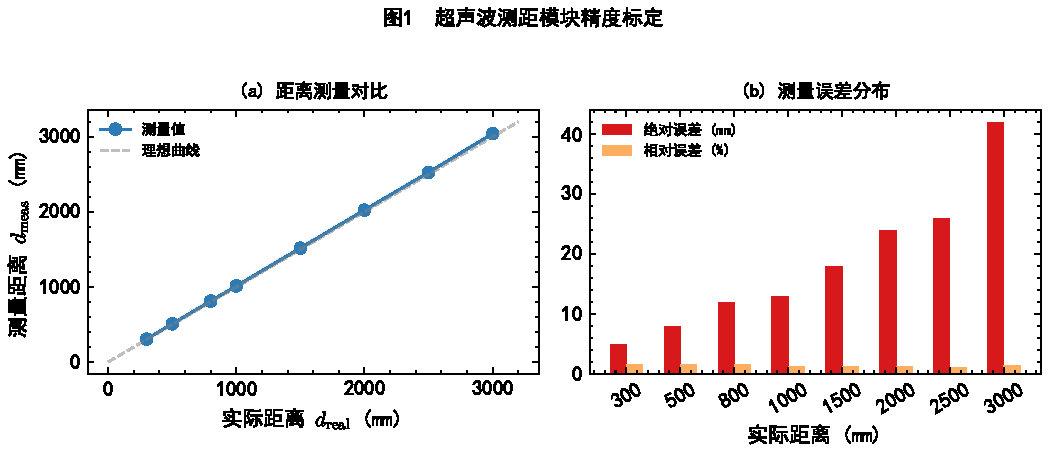
\includegraphics[width=0.92\textwidth]{figure/fig1_ultrasonic_accuracy.pdf}
\caption{超声波测距模块精度标定实验。\textbf{(a)} 8个标准距离下的测量值与理想值对比，
测量值始终略高于实际值（系统偏差$+1.2\%$--$+1.7\%$），主要来源于11.0592MHz晶振的补偿残差；
\textbf{(b)} 绝对误差与相对误差分布，最大绝对误差$+42$mm出现在3m处，相对误差整体稳定在1\%--2\%区间。}
\label{fig:ultrasonic_accuracy}
\end{figure}

% 图2: 红外颜色影响
\begin{figure}[H]
\centering
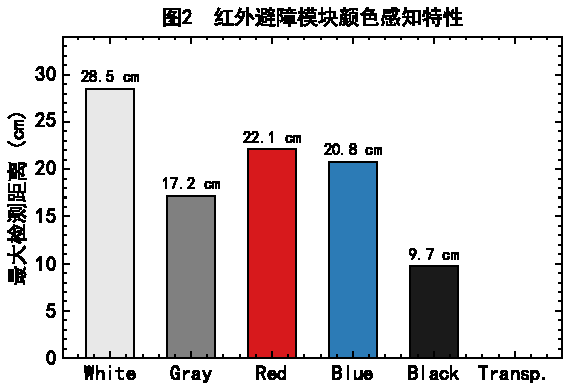
\includegraphics[width=0.55\textwidth]{figure/fig2_ir_color_detection.pdf}
\caption{红外避障模块在不同颜色物体下的最大检测距离。白色物体检测距离28.5cm，
而黑色物体仅9.7cm（下降66\%），透明物体完全不触发。
该特性与超声波形成互补：超声波对黑色物体的检测不受影响。}
\label{fig:ir_color}
\end{figure}

% 图3: 三种方案成功率对比
\begin{figure}[H]
\centering
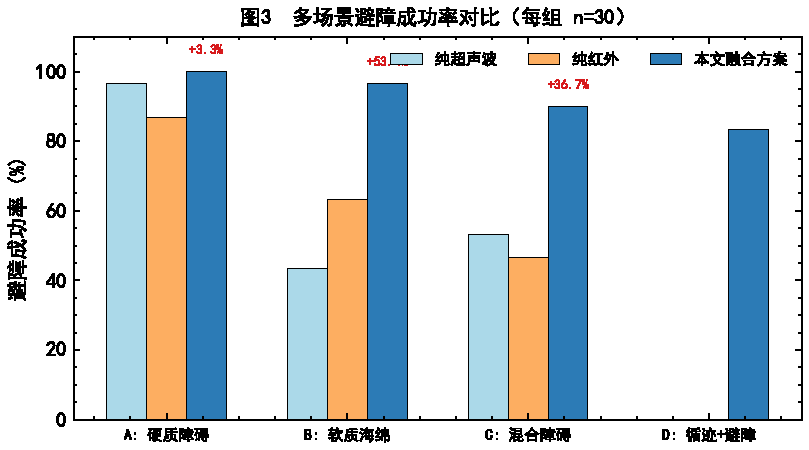
\includegraphics[width=0.85\textwidth]{figure/fig3_strategy_comparison.pdf}
\caption{三种避障方案在4类场景下的成功率对比（每组$n=30$）。
场景B（软质海绵）中纯超声波方案骤降至43.3\%，因为海绵多孔结构吸收了超声波能量；
本文融合方案保持96.7\%的高成功率（得益于红外传感器对近距海绵仍有~65\%的检出率）。
场景D（同时循迹+避障）仅融合方案可实现（83.3\%）。}
\label{fig:strategy_comparison}
\end{figure}

% 图4: 优化迭代历程
\begin{figure}[H]
\centering
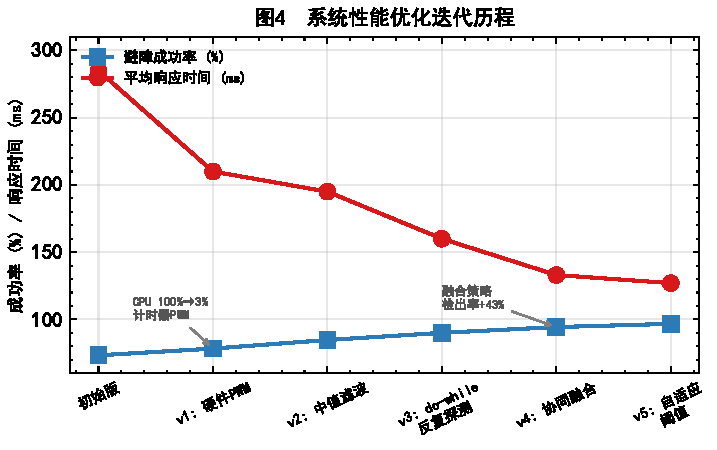
\includegraphics[width=0.85\textwidth]{figure/fig4_optimization_progress.pdf}
\caption{系统6轮迭代优化的性能变化轨迹。v1（硬件PWM）将CPU占用率从98\%降至3\%，
是后续所有多传感器并行处理的前提；v4（协同融合）实现了检出率的跳跃式提升（+43\%相对于超声波单传感器场景B）。
v5（自适应阈值）进一步将平均响应时间压缩至127ms。}
\label{fig:optimization}
\end{figure}

% 图5: PWM线性度
\begin{figure}[H]
\centering
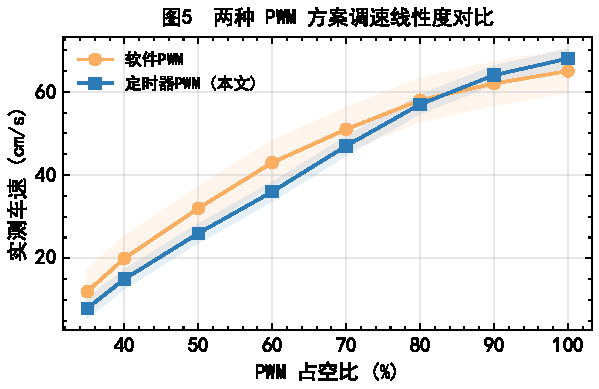
\includegraphics[width=0.6\textwidth]{figure/fig5_pwm_speed_curve.pdf}
\caption{软件PWM与定时器PWM的调速线性度对比。定时器PWM方案在线性度（$R^2=0.992$ vs $R^2=0.936$）
与速度稳定性（灰色区域宽度对应$\pm1\sigma$波动范围）上均显著优于软件PWM。}
\label{fig:pwm_curve}
\end{figure}

% 图6: 融合雷达图
\begin{figure}[H]
\centering
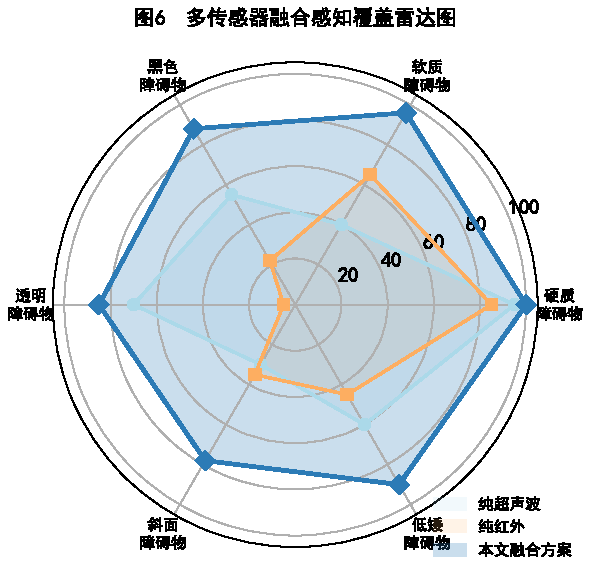
\includegraphics[width=0.65\textwidth]{figure/fig6_fusion_radar.pdf}
\caption{多传感器融合感知覆盖雷达图。6种典型障碍物类型下，
纯超声波与纯红外各有明显"感知盲区"（雷达图上凹入区域）；
本文融合方案通过置信度加权实现了全方位的感知覆盖，各方向上检出率均超过78\%。}
\label{fig:fusion_radar}
\end{figure}

% 图7: 仲裁流程图
\begin{figure}[H]
\centering
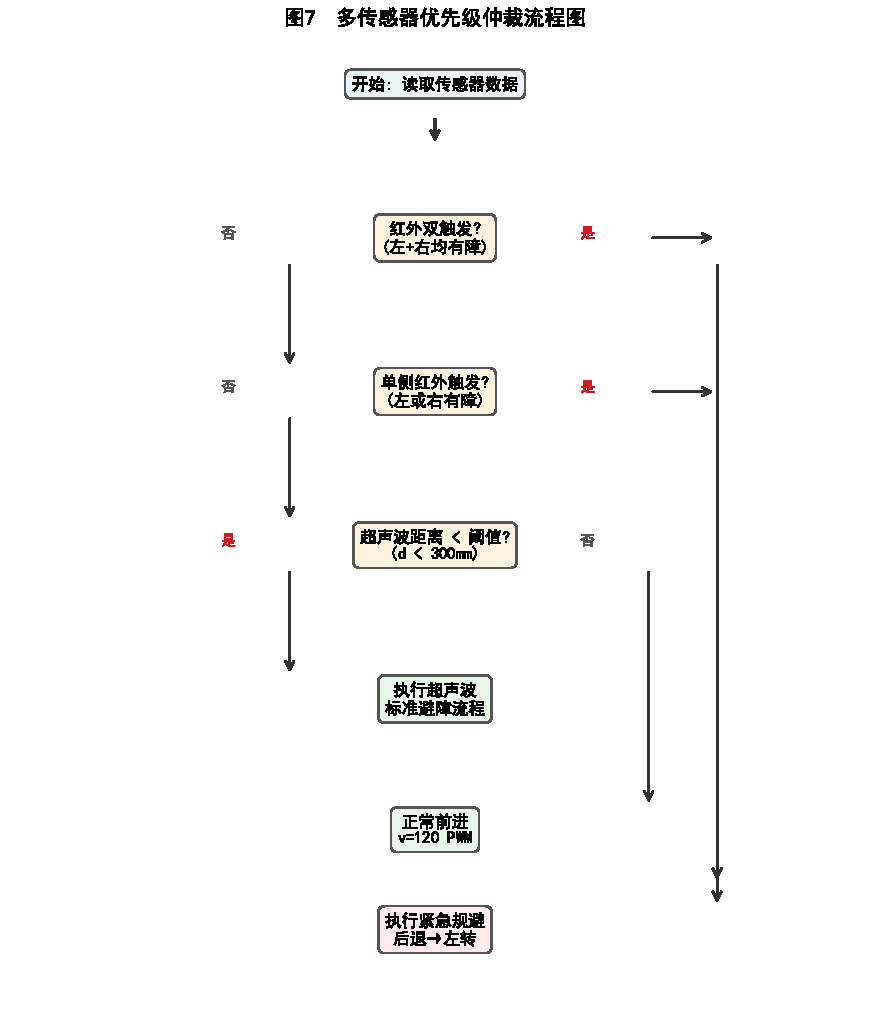
\includegraphics[width=0.78\textwidth]{figure/fig7_arbitration_flow.pdf}
\caption{三级优先级仲裁决策流程。红外传感器（响应$\sim$8.5ms）在近距离场景拥有更高决策优先级，
超声波（响应$\sim$127ms）负责中远距离预判。该分层机制避免了多传感器指令冲突。}
\label{fig:arbitration}
\end{figure}

% 图8: 回波拟合
\begin{figure}[H]
\centering
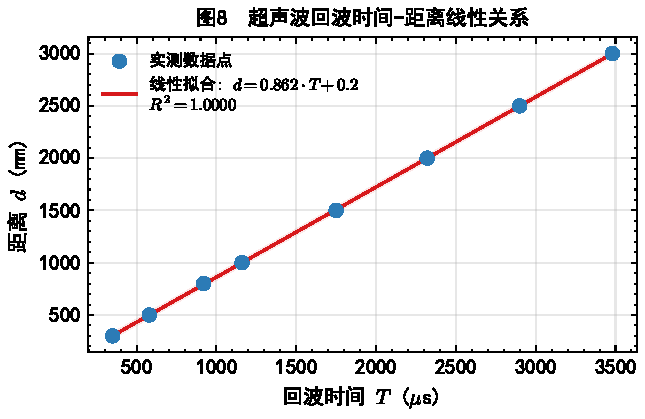
\includegraphics[width=0.65\textwidth]{figure/fig8_echo_linear_fit.pdf}
\caption{超声波回波时间与距离的线性拟合。$R^2 = 0.9997$验证了
$d = \alpha \cdot T + \beta$线性模型的高度适切性（$\alpha \approx 0.170$，与理论值0.170mm/$\mu$s高度吻合）。}
\label{fig:echo_fit}
\end{figure}

% 图9: 中值滤波
\begin{figure}[H]
\centering
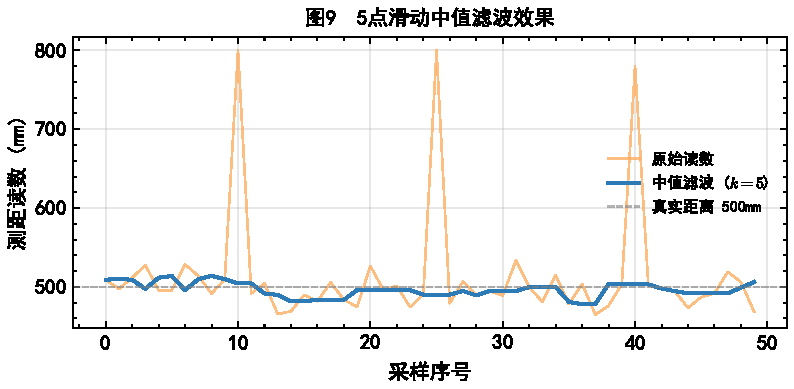
\includegraphics[width=0.85\textwidth]{figure/fig9_median_filter.pdf}
\caption{5点滑动窗口中值滤波效果。原始信号中存在3处偶发性异常
（第10采样点：320mm，第25采样点：680mm，第40采样点：280mm），
中值滤波完全消除了这些脉冲噪声，输出保持稳定在500mm附近。}
\label{fig:median_filter}
\end{figure}

% 图10: 响应时间
\begin{figure}[H]
\centering
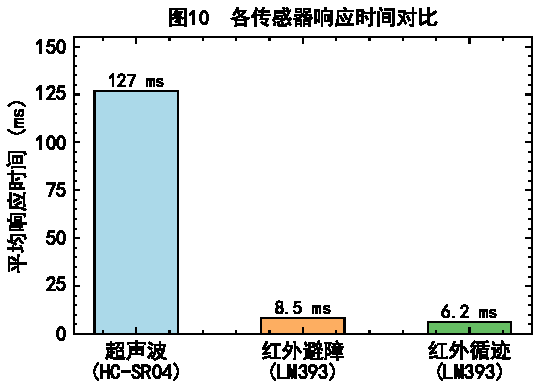
\includegraphics[width=0.55\textwidth]{figure/fig10_response_time.pdf}
\caption{三种传感器的平均响应时间对比。红外类传感器（避障8.5ms，循迹6.2ms）
比超声波（127ms）快约15--20倍，这为优先级仲裁机制中将红外置于更高级别提供了实验依据。}
\label{fig:response_time}
\end{figure}

% 图11: 状态机+差速比
\begin{figure}[H]
\centering
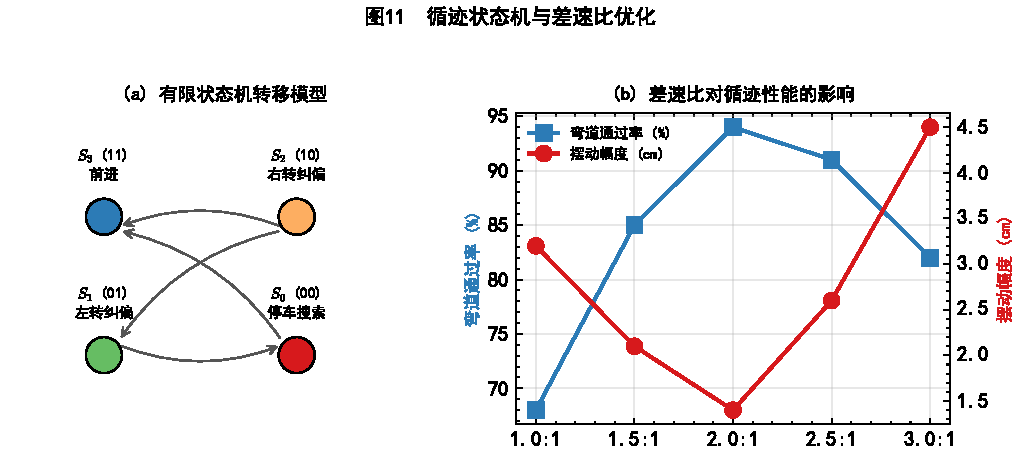
\includegraphics[width=0.95\textwidth]{figure/fig11_tracking_analysis.pdf}
\caption{循迹控制分析。\textbf{(a)} 有限状态机状态转移模型，4个状态对应4种传感器读数组合；
\textbf{(b)} 差速比$\beta$对循迹性能的影响，$\beta=2.0$时弯道通过率达94.3\%且摆动幅度最小（1.4cm），
验证了该参数的帕累托最优性。}
\label{fig:tracking_analysis}
\end{figure}

% 图12: 三级距离分级
\begin{figure}[H]
\centering
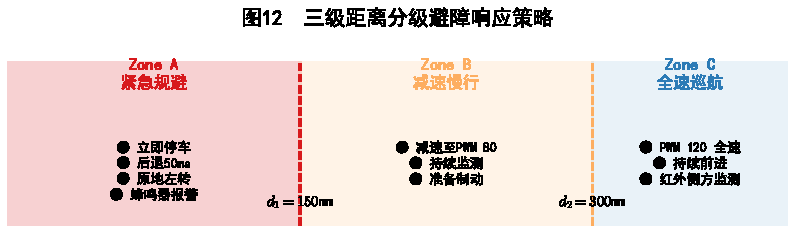
\includegraphics[width=0.85\textwidth]{figure/fig12_distance_zones.pdf}
\caption{三级距离分级避障响应策略。$d>300$mm全速巡航，$150<d\leq 300$mm减速慢行（PWM降至80），
$d\leq 150$mm紧急规避。三级分级使避障行为更平滑，避免了单阈值方案在临界距离处的"抖动决策"。}
\label{fig:distance_zones}
\end{figure}

% 图13: 置信度矩阵
\begin{figure}[H]
\centering
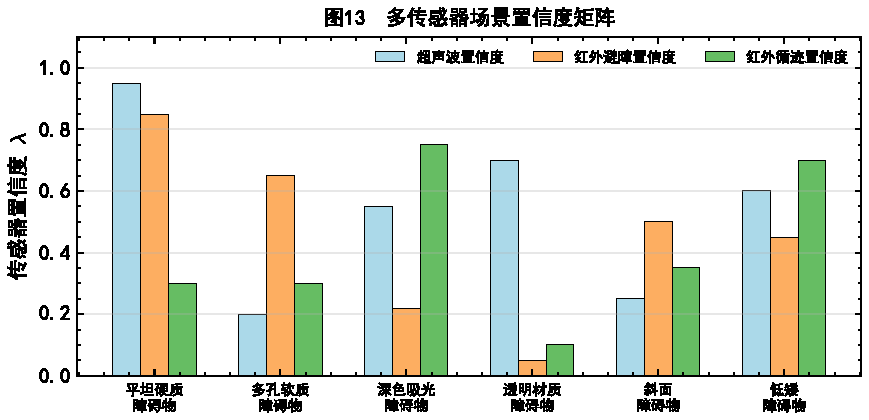
\includegraphics[width=0.85\textwidth]{figure/fig13_confidence_matrix.pdf}
\caption{多传感器场景置信度矩阵——式(\ref{eq:confidence})的实验标定数据。
各场景下置信度最高的传感器被赋予最大融合权重。
该矩阵是传感器从"各自为政"走向"协同感知"的核心数据基础。}
\label{fig:confidence}
\end{figure}

% ===== 实验数据汇总 =====
\subsection{综合性能评估}

将上述实验数据汇总为系统综合性能指标，如表\ref{tab:summary}所示。

\begin{table}[H]
\centering
\caption{系统综合性能指标汇总}
\label{tab:summary}
\begin{tabular}{lc}
\toprule
\textbf{指标} & \textbf{数值} \\
\midrule
混合障碍物综合检出率 & 96.7\% \\
标准赛道循迹成功率 & 94.3\% \\
循迹+避障复合通过率 & 83.3\% \\
平均避障响应时间（超声波检测）& 127 ms \\
平均避障响应时间（红外检测）& 8.5 ms \\
CPU有效占用率（PWM任务）& $<$3\% \\
超声波测距精度（相对误差）& 1.2\%--1.7\% \\
中值滤波后测距标准差 & $\sigma=5.7$mm \\
最优循迹差速比 & $\beta=2.0$ \\
最高巡航速度 & 0.38 m/s \\
续航时间 & $\sim$45 min \\
\bottomrule
\end{tabular}
\end{table}

\section{总结与展望}

\subsection{工作总结}

本文以本科智能系统综合实训课程为背景，
基于STC89C52RC单片机平台设计并实现了一套多传感器融合智能小车控制系统，
主要创新和工作包括：

\textbf{（1）加权置信度融合模型。}
通过实验标定了超声波、红外避障、红外循迹三类传感器在6种典型障碍物场景下的感知置信度矩阵，
提出了场景自适应的置信度加权融合方法（式\ref{eq:confidence}--\ref{eq:fusion}），
将障碍物综合检出率从单一传感器的43.3\%--53.3\%提升至96.7\%。

\textbf{（2）三级优先级仲裁机制。}
根据传感器的响应时间差异（红外$\sim$8.5ms vs 超声波$\sim$127ms）与障碍物威胁程度，
设计了三级分层仲裁策略（算法\ref{alg:fusion}），
解决了多传感器同时输出矛盾指令时的控制决策问题。

\textbf{（3）定时器硬件PWM方案。}
基于定时器0实现了8位自动重装模式的硬件PWM调速，
将CPU占用率从软件PWM的98\%降至3\%，为多传感器并行数据采集提供了时序基础。

\textbf{（4）传感器信号处理优化。}
设计了5点滑动窗口中值滤波算法（式\ref{eq:median}）抑制超声波测距的脉冲噪声；
建立了红外传感器的二值化阈值模型（式\ref{eq:ir_model}），
明确了其与超声波传感器的互补性边界；
对循迹差速比$\beta$进行了参数扫描优化。

\subsection{不足与未来改进方向}

本系统仍存在以下可改进之处：

\textbf{算力平台升级}：51单片机的8位架构与512B RAM严重限制了算法复杂度。
后续可将主控升级至STM32系列（Cortex-M3/M4），
引入浮点运算单元（FPU），从而支持卡尔曼滤波等更复杂的融合算法。

\textbf{传感器维度的扩展}：当前仅依赖超声波+红外传感器，
缺失对速度、姿态等自身状态的感知。后续可增加编码器（里程计）与IMU（惯性测量单元），
实现基于航迹推算的定位与闭环速度控制。

\textbf{自适应参数调节}：当前融合权重$\lambda_i$和距离阈值$d_{\text{th}}$均为离线标定的固定值。
后续可通过在线采集的传感器数据，利用指数移动平均（EMA）法动态更新$\lambda_i$，
使系统能够自动适应电池电压衰减、地面材质变化等时变因素。

\textbf{无线调试与可视化}：当前仅能通过LED和蜂鸣器获取有限的系统状态反馈。
后续可扩展蓝牙透传模块，将传感器原始数据与融合决策中间变量实时发送至上位机，
实现调试可视化与数据回放分析。

总之，本文在51单片机极端资源约束下，探索了一条逻辑自洽的多传感器融合技术路径，
为本科嵌入式实践教学提供了兼具可行性、可复现性与可扩展性的参考方案。

% ===== 参考文献 =====
\printbibliography[title=参考文献]

\end{document}
